% (c) GreenSocs Ltd 2008
% author: Christian Schroeder <schroeder@eis.cs.tu-bs.de>

%%%%%%%%%%%%%%%
\section{Output Plugins}
\label{GAVOutputPlugins}

{\em Output plugins} are used to export any \lstinline|gs_param| value over time to a specific output. Such outputs can be the stdout, text-files, csv-files, SCV streams, dedicated connections to tools, e.g. TCP/IP connections etc. (see Figure \ref{fig:GAVConceptOutputs}).

Each output plugin is able to output multiple \lstinline|gs_param|s which can be added to the output during simulation runtime by a user or a tool. The only assumption is to have access to a GAV User API (see section \ref{GAVUserAPI}).

Before you are able to use one or more output plugin(s), you have to include the one(s) you need:

\noindent
\begin{minipage}{\textwidth}
\begin{lstlisting}[caption={Include for output plugin}, label=lst:GAVIncludeOutputPlugin]
// e.g.
#include "greencontrol/analysis.h" // includes the Standard Output Plugin
#include "greencontrol/analysis_file_outputplugin.h"
#include "greencontrol/analysis_csv_outputplugin.h"
#include "greencontrol/analysis_scv_outputplugin.h"
// etc.
\end{lstlisting}
\end{minipage}

\begin{figure}[htbp]
	\centerline{
		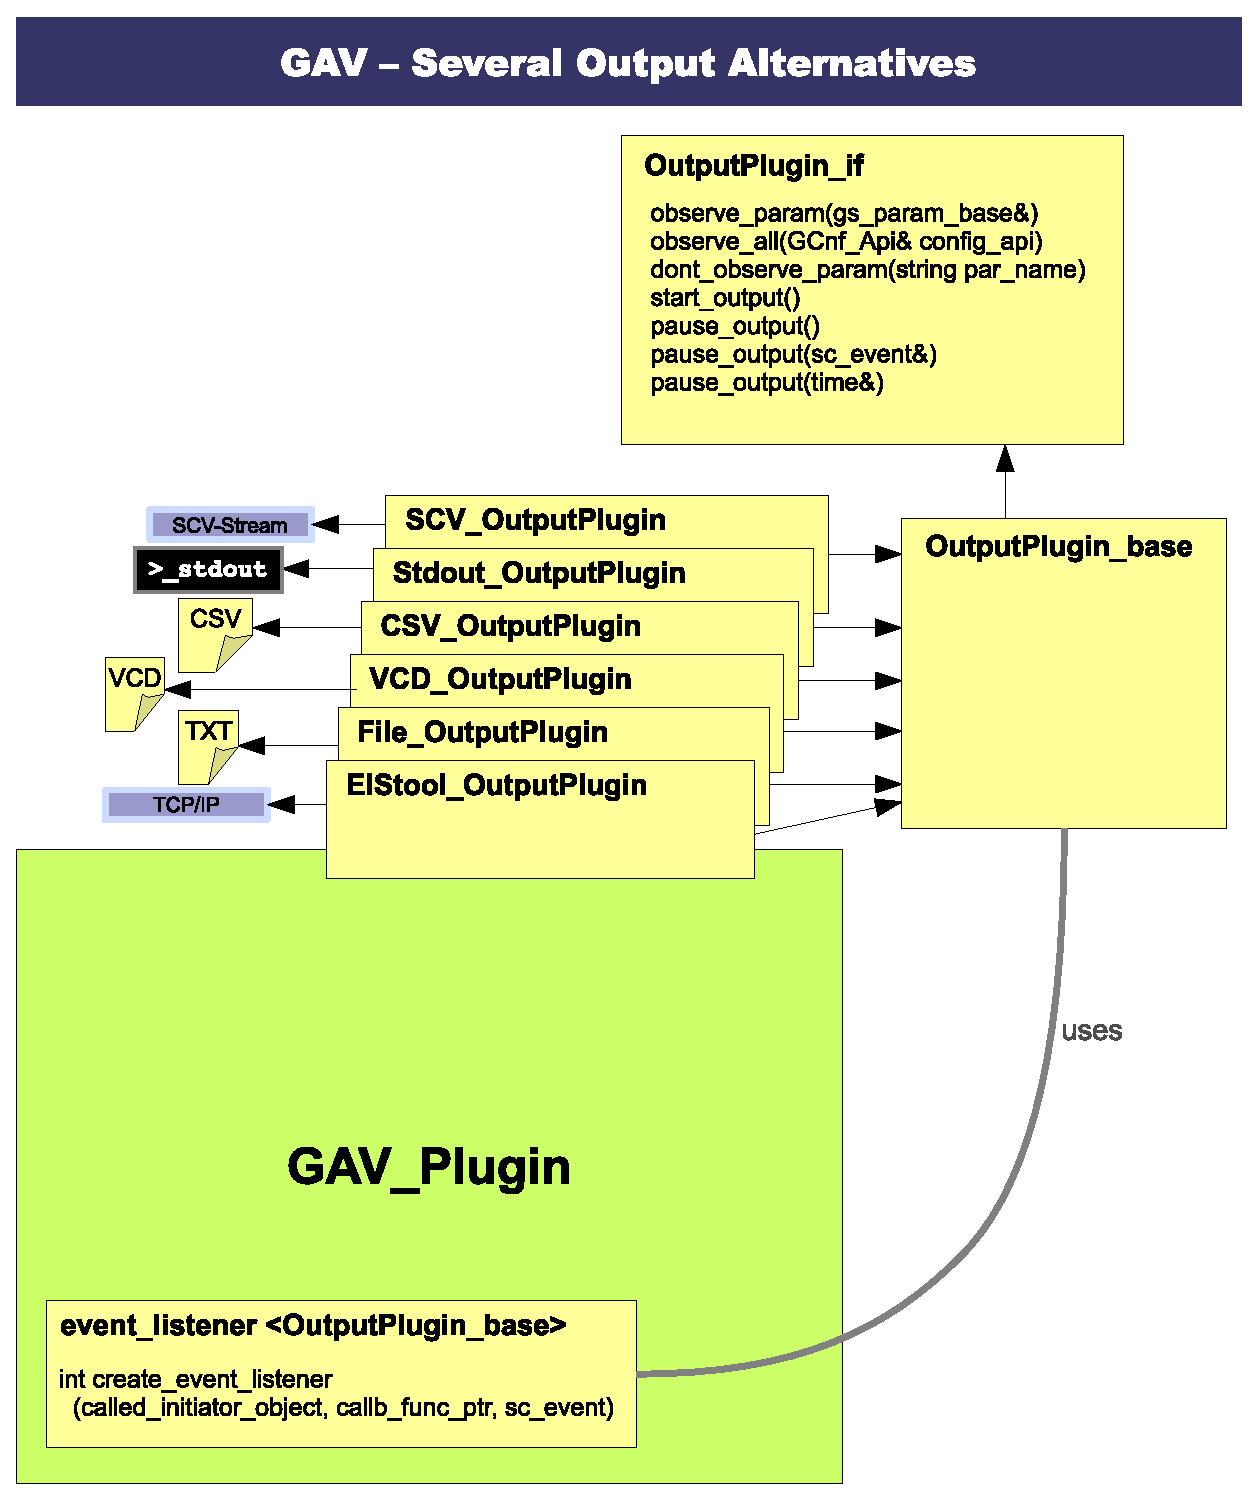
\includegraphics[width=12cm]{./images/GAVconcept(Outputs)}}
	\caption{GreenAV Concept for Outputs: The \lstinline|GAV_Plugin| contains several types of output plugins}
	\label{fig:GAVConceptOutputs}
\end{figure}


%%%
\ZwischenUberschrift{Default Output Plugin(s)} 
The provided output plugins are described in the following subsections. Any output plugin existing in the simulation is owned by the GAV plugin. For each type of output plugin there is one {\em default instance} which should be used if (only) one instance (instead of multiple ones) meets the user's requirements. A simulation-wide default output plugin type (which results in a default instance) should be set by the user during construction. If more than the default output(s) is needed (e.g. if several files should be created) the user may create {\em additional instances} of each output plugin type.

Specify the simulation-wide default output plugin like shown in listing \ref{lst:GAVDefaultOutputPlugin}. All outputs that are not directed to a special type or instance will use this default output plugin.

The output plugin types are identified with the type {\sffamily gs::gav::OutputPluginType} (which is an unsigned int). For convenience their names can be used instead. See the following sections of each output plugin for its value. {\sffamily DEFAULT\_OUT} is used as a replacement for the simulation-wide default.

\noindent
\begin{minipage}{\textwidth}
\begin{lstlisting}[caption={Specify the default output plugin during Analysis Plugin instantiation}, label=lst:GAVDefaultOutputPlugin]
gs::av::GAV_Plugin analysisPlugin("AnalysisPlugin", gs::av::STDOUT_OUT);
\end{lstlisting}
\end{minipage}

\WarningSymbol{} Only if you know what you are doing, you may use the GAV Plugin function \newline \lstinline[language=TeX]|void set_default_output_plugin(OutputPluginType default_output_plugin_type)| \newline
to modify the default output plugin even during model creation and simulation.

See next paragraph and section \ref{GAVUserAPI} for how to access default output plugins and how to create and access additional ones.

\Note{Implementation Note}{Output Plugin identification}{
  The output plugins are identified (id) using the {\sffamily unsigned int OutputPluginType}. A static map {\sffamily OutPluginName::getMap()} is used to store the names (values) related to the id (key).
  
  A variable of type {\sffamily OutputPluginType}, named as the output plugin name, with the corresponding value can be used to identify the type using  {\sffamily gs::av::TXT\_FILE\_OUT} etc. 
}

%%%%
\ZwischenUberschrift{Access Output Plugins}\hypertarget{AccessOutputPlugins}
Before using an output plugin the user needs to get a default instance or create a new one. Use the GAV user API (see section\ref{GAVUserAPI}). Several functions are available to access output plugins. See the code example for an example how to use.

\begin{itemize}
  \item Recommended way accessing the default output plugin of the needed type: \newline
     Get the default output plugin by calling
     \lstinline[language=TeX]|OutputPlugin_if* get_default_output(const OutputPluginType type = DEFAULT_OUT)|.
     If the module does not care about the output type, leave the type empty which will return the simulation-wide default output plugin. The returned output plugin pointer can be used to add parameters for observation or to control it (see section \hyperlink{InterfaceAndHowToUse}{Interface and how to use}).

  \item When needing further output plugin instances, a call of \lstinline|OutputPlugin_if* create_OutputPlugin (OutputPluginType, string ctor_par)| will create a new instance using the string as constructor parameter (e.g. filename). The user should store the returned pointer to be able to add parameters using the function \lstinline|add_to_output| (see below).
  
\end{itemize}


%%%%
\ZwischenUberschrift{Observing Parameters with Output Plugins}
There are two basically different ways adding a parameter for observation to an output plugin: One way is calling GAV user API functions. This assumes you have pointer access to the output plugin instance and the parameter (which is no issue within the simulation). Another way is creating and manipulating parameters belonging to special output plugins. For this you need to know the name of the output plugin you want to observe a parameter and the name of the parameter.

{\em Manipulate output plugins directly}:
\begin{itemize}
	\item See section \hyperlink{InterfaceAndHowToUse}{Interface and how to use} for various actions possible on output plugin pointers that you got by calling \lstinline|get_default_output| or creating new ones (see section \hyperlink{AccessOutputPlugins}{Access Output Plugins}).
\end{itemize}

Observe parameters by {\em calling GAV user API functions}:
\begin{itemize}
  \item Adding a parameter for observation to a default or manually created output plugin can be done using the function
      \mbox{\lstinline|OutputPlugin_if* add_to_output(OutputPlugin_if*, gs_param_base*)|.} The output plugin (first parameter) is one of the pointers returned by the functions above (\lstinline|get_default_output| and \lstinline|create_outputPlugin|).
  
  \item Another way observing a parameter with one of the default plugins is calling \lstinline|OutputPlugin_if* add_to_default_output(OutputPluginType, gs_param_base*)| which adds a parameter to the default instance of the specified type. It returns a pointer to the default output plugin, too.
  
  \item The easiest way observing a parameter with the simulation-wide default output is calling 
  	the function \lstinline|OutputPlugin_if* add_to_default_output(gs_param_base*)|. It returns 
	a pointer to the default output plugin, too.
\end{itemize}

Observe parameters by {\em creating and manipulating parameters belonging to special output plugins}:
\begin{itemize}
  \item To enable the observation of a parameter (which may be already existing or may not), create a new implicit parameter which is a child parameter of the output plugin and is named as the parameter that should be observed. This comes clear in the following example:
	\begin{itemize}
  		\item The GAV Plugin is named ``{\sffamily AnalysisPlugin}''.
  		\item The output plugin which should observe the parameter is the default stdout one, automatically named \mbox{``{\sffamily STDOUT\_OUT\_default}''}.
		\item The parameter that should be observed is named ``{\sffamily mymodule.submodule.myparam}''.
		\item To observe the parameter with the output plugin, simply create a so-called {\em enabled parameter} (child of the output plugin) named \mbox{``{\sffamily AnalysisPlugin.STDOUT\_OUT\_default.mymodule.submodule.myparam}''} by doing the following call on the config user API:  
		\begin{lstlisting}
mCnfApi->setInitValue("AnalysisPlugin.STDOUT_OUT_default.mymodule.submodule.myparam", "true");
		\end{lstlisting}
		The output plugin will automatically make the implicit parameter explicit immediately.
		\item Afterward you can enable and disable the observation of the parameter by modifying the 'enabled parameter' to true or false, e.g. 
		\begin{lstlisting}
gs::gs_param<bool> *enabled
  = mCnfApi->get_gs_param<bool>("AnalysisPlugin.STDOUT_OUT_default.mymodule.submodule.myparam");
*enabled = false;
		\end{lstlisting}
	\end{itemize}

This works as well with any manually created output plugin. E.g. to add a parameter to an output plugin named \mbox{``{\sffamily mymodule.main\_action.STDOUT\_OUT\_userChosenConstructorParam}''} this is done by calling
		\begin{lstlisting}
mCnfApi->setInitValue("mymodule.main_action.STDOUT_OUT_userChosenConstructorParam.mymodule.param2", "true");
		\end{lstlisting}

\end{itemize}


%%%%
\ZwischenUberschrift{Output Plugin Names}
An output plugin is an {\sffamily sc\_object} which is named in the following pattern. The name is needed e.g. when creating 'enabled parameters' (see above) for this output plugin.

All output plugin names have their name string as prefix (e.g. {\sffamily STDOUT\_OUT}) and their constructor parameter as tail.

The default output plugins (one for each available output plugin type) are created and owned by the GAV Plugin. Their name tails are {\sffamily \_default} (which is the constructor parameter specified by the GAV Plugin).

The tail is automatically converted to SystemC conform names by replacing each character which is not a letter or a digit or an underscore to an underscore.

Examples:
\begin{itemize}
	\item {\em Default} output plugin of type {\sffamily STDOUT\_OUT}: \newline 
	name: {\sffamily AnalysisPlugin.STDOUT\_OUT\_default}
	\item {\em Default} output plugin of type {\sffamily TXT\_FILE\_OUT}: \newline
	name: {\sffamily AnalysisPlugin.TXT\_FILE\_OUT\_default}
	\item User created output plugin created {\em in the constructor} of module {\sffamily mymodule} with the call \lstinline|create_OutputPlugin(TXT_FILE_OUT, "myop")|: \newline
	name: {\sffamily mymodule.TXT\_FILE\_OUT\_myop}
	\item User created output plugin created {\em in the constructor} of module {\sffamily mymodule} with the call \lstinline|create_OutputPlugin(TXT_FILE_OUT, "myop.txt")|: \newline
	name: {\sffamily mymodule.TXT\_FILE\_OUT\_myop\_txt}
	\item User created output plugin created {\em in the thread} {\sffamily main\_action} of module {\sffamily mymodule} with the call \lstinline|create_OutputPlugin(TXT_FILE_OUT, "myop.txt")|: \newline
	name: {\sffamily mymodule,main\_action.TXT\_FILE\_OUT\_myop\_txt}
\end{itemize}

%%%
\ZwischenUberschrift{Interface and how to use}\hypertarget{InterfaceAndHowToUse}
After the user got an output plugin pointer of type \lstinline|OutputPlugin_if| (see \Datei{OutputPlugin\_if}) it may be used: Call

\begin{itemize}
  \item \lstinline|observe(gs_param_base&)| to let the output plugin observe a parameter.
  \item \lstinline|observe_all(GCnf_Api& config_api)| to observe all parameters currently existing.
  \item \lstinline|observe(vector<gs_param_base*>)| to observe parameters given in a vector (e.g. as a result of the config user API call \lstinline|getParams(string)|).
  \item \lstinline|observe(string getParamList_string)| to observe parameters specified by a string like \mbox{``\sffamily myModule.*}''. Internally the config API call \lstinline|getParams(string)| will be used. To observe all parameters underneath the hierarchy level of {\sffamily myModule}, call \lstinline|observe("myModule.*")|.
  \item \lstinline|remove(gs_param_base&)| to remove a parameter observation from the output.
  \item \lstinline|pause()| to pause the output from now on.
  \item \lstinline|pause(sc_event&)| to pause the output until the given event is notified.
  \item \lstinline|pause(sc_time&)| or \lstinline[language=TeX]|pause(double, sc_time_unit)| to pause the output for the given time.
  \item \lstinline|resume()| to resume the output manually if paused.
\end{itemize}

Consult the doxygen API \footnote{\hypertarget{GAVDoxygenRef08target}{\GreenAV doxygen API}: \url{http://www.greensocs.com/projects/GreenControl/GreenAV/docs/GreenAVDoxygen} (take care to look at the correct release)} for more details.

An output plugin is not paused by default.

The usage of output plugins is shown in the example \Verzeichnis{greencontrol/examples/gav\_simple}, especially in the files \Datei{AVAnalyserTool.*}.

The type of output plugins is defined with an enum {\sffamily OutputPluginType} (see file \mbox{\Datei{gav\_datatypes.h}).}

\noindent
\begin{minipage}{\textwidth}
\paragraph{Code example}
Listing \ref{lst:GAVOuputExample} and figure \ref{fig:GAVOutputExample} show examples how to use output plugins.

\begin{lstlisting}[caption={Output plugin code example}, label=lst:GAVOuputExample]
// get pointer to parameter bases
gs::gs_param_base *int_par  = m_configAPI.getPar("Owner.int_param");
gs::gs_param_base *str_par  = m_configAPI.getPar("Owner.str_param");
gs::gs_param_base *uint_par = m_configAPI.getPar("Owner.uint_param");

// get simulation-wide default output, and observe a param
gs::av::OutputPlugin_if* overallDefaultOP = m_analysisAPI.get_default_output();
m_gavApi.add_to_output(overallDefaultOP, int_par);
// alternative: add params to the default text file output  
gs::av::OutputPlugin_if* fileOP =
    m_gavApi.add_to_default_output(gs::av::TXT_FILE_OUT, int_par);
m_gavApi.add_to_default_output(gs::av::TXT_FILE_OUT, uint_par);

// create an additional CSV-file output plugin and add all existing
// parameter to output
gs::av::OutputPlugin_if* csvFileOP = 
    m_gavApi.create_OutputPlugin(gs::av::CSV_FILE_OUT, "CSVexp.log");
csvFileOP->observe_all(m_configAPI);

// pause for 2 ns.
csvFileOP->pause(2, SC_NS);

// remove parameter from default file output
fileOP->remove(*int_par);
\end{lstlisting}
\end{minipage}

\begin{figure}[ht]
	\centerline{
		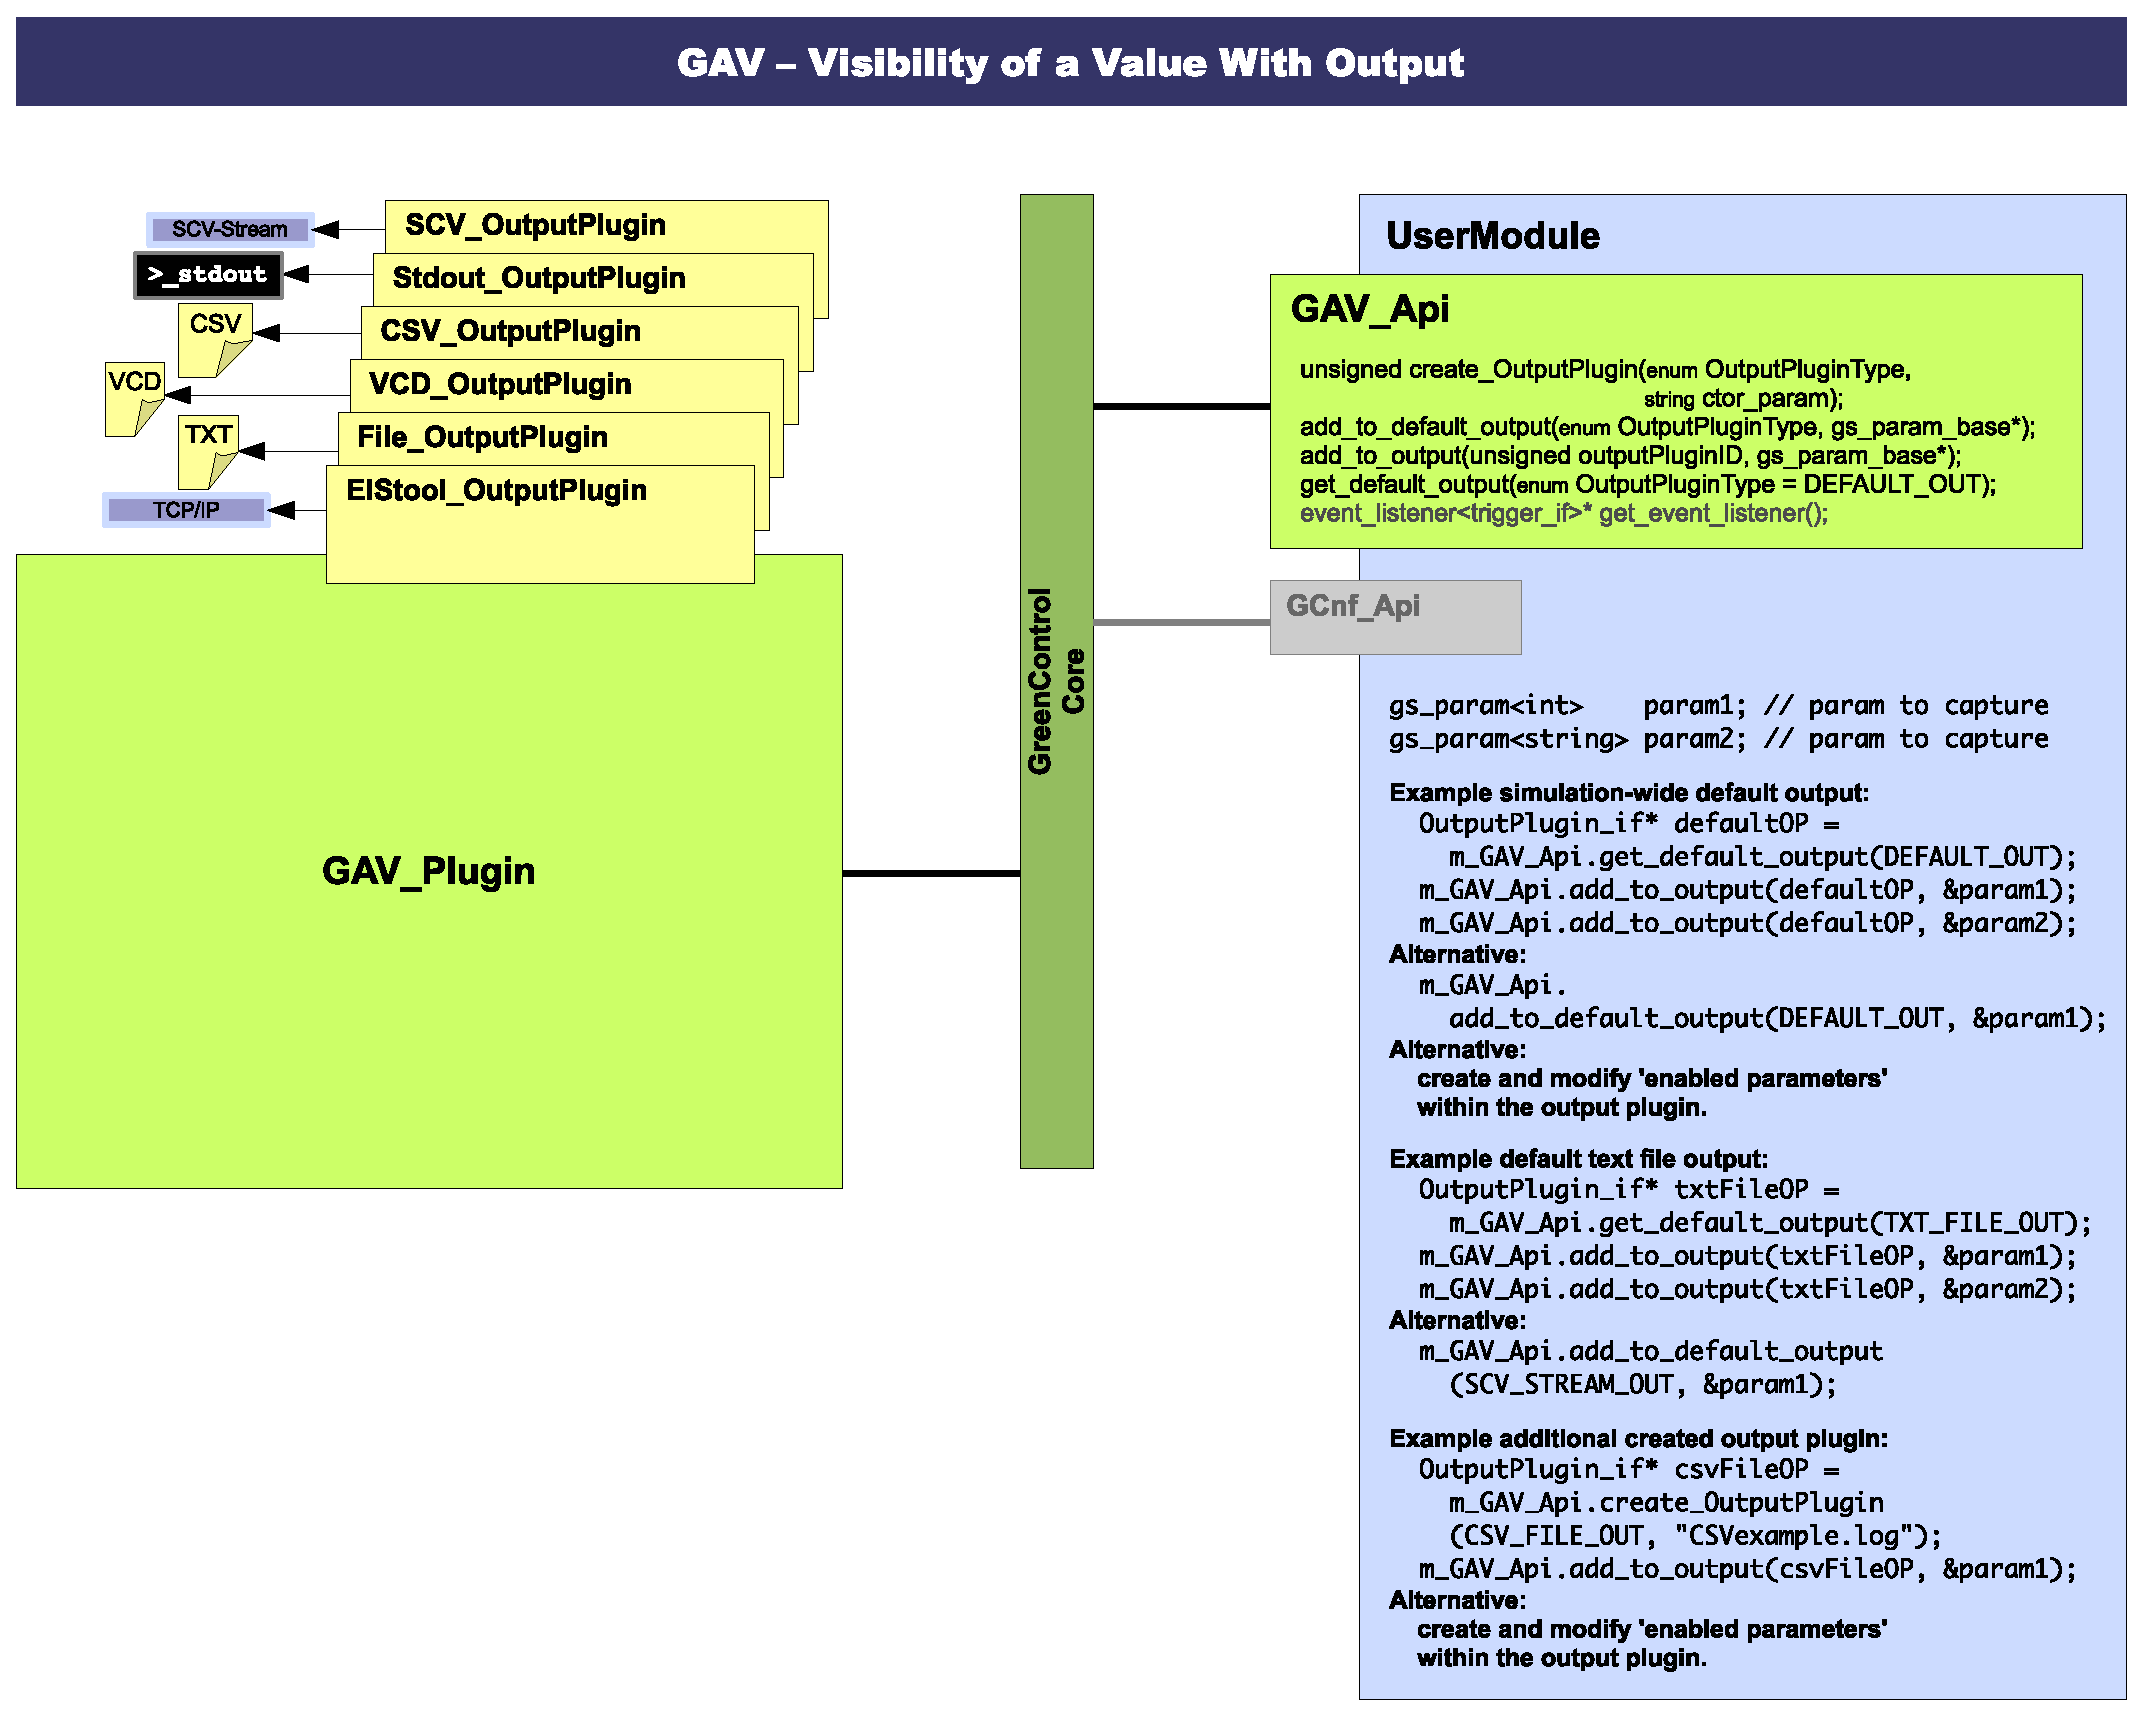
\includegraphics[width=\linewidth]{./images/GAVconcept(OutputExample)}}
	\caption{GreenAV Output Example}
	\label{fig:GAVOutputExample}
\end{figure}


\Note{Implementation Note}{Output Plugin}{
  The output plugin instances are newed by the GAV plugin and stored in two maps: one for the 
  default (\lstinline|m_DefaultOutputPlugins|) and one for the additional (\lstinline|m_OutputPlugins|) output plugins.
  
  One event listener (\lstinline|m_OutpPl_event_listener|, see section \ref{GAVEventListener}) is owned by the GAV plugin to handle events (pause and resume) of output plugins.
}

\Note{Implementation Note}{OutputPlugin\_base}{
 An output plugin derives from the base class \lstinline|OutputPlugin_base| (see file \Datei{OutputPlugin\_base}).\\

 Each output plugin needs only implement its constructor, destructor, the initialization function \lstinline|init()| and
 the callback function \lstinline|config_callback| which should perform the actual output.

 Output plugins implement the constructor which gets one string parameter
 to allow adding the output plugin to the GAV plugin's create command.
 
 All functions are virtual to give the derived class the oportunity to catch the
 calls before calling the base class' function. \\

 The derived classes need to call \lstinline|init()| on the first access (dependent on the variable \lstinline|bool is_used|), not during construction. The constructor should not do memory allocations etc. because it is called (for the default output plugins) even if the output plugin will never be used.
}


%%%%
\subsection{Default Output Plugin (special case)}
\label{GAVOPdefault}

\begin{itemize}
  \item Identify the default output plugin (which is actually one of the following) with \newline
  	{\sffamily gs::av::DEFAULT\_OUT}, \newline
           id ({\sffamily OutputPluginType}) = 0.
\end{itemize}

%%%%
\subsection{NULL Output Plugin (special case)}
\label{GAVOPnull}

\begin{itemize}
  \item Identify the NULL output plugin (which is actually no one) with \newline
  	{\sffamily gs::av::NULL\_OUT}, \newline
           id ({\sffamily OutputPluginType}) = 1.
\end{itemize}

Use this setting if the output should go nowhere.

%%%%
\subsection{STDOUT Output Plugin}
\label{GAVOPstdout}

\begin{itemize}
  \item Included within \Datei{greencontrol/analysis.h}
  \item Implementation see file \Datei{Stdout\_OutputPlugin.h}
  \item Identify this output plugin with {\sffamily gs::av::STDOUT\_OUT}, \newline
           id ({\sffamily OutputPluginType}) = 3.
\end{itemize}

The STDOUT output plugin can be used to simply display parameter changes to the standard output (e.g. terminal where the simulation runs).

One line per parameter change is printed and contains timing (and delta) information, the parameter name and the new value. An output example can be seen in listing \ref{lst:stdoutOutputPluginEx}.

This output plugin is a very convenient way to print each parameter change to the simulation output.

The constructor string parameter is not used within this output plugin.

\begin{lstlisting}[caption={STDOUT output example}, label=lst:stdoutOutputPluginEx]
@130 ns /7 (Stdout_OutputPlugin): AVnewStatCalc.int_par = 2
\end{lstlisting}


%%%%
\subsection{Text-file Output Plugin}
\label{GAVOPfile}

\begin{itemize}
  \item Include \Datei{greencontrol/analysis\_file\_outputplugin.h}
  \item Implementation see file \Datei{File\_OutputPlugin}
  \item Identify this output plugin with {\sffamily gs::av::TXT\_FILE\_OUT}, \newline
           id ({\sffamily OutputPluginType}) = 2.
\end{itemize}

The Text-file output plugin can be used to record parameter changes to a human-readable text file. The format is similar to the STDOUT plugin's output: The first line is the simulation time, the following lines contain one line per parameter change. See listing \ref{lst:fileOutputPluginEx} for an example.

The constructor parameter is the filename of the output file. Be careful to set the file extension (e.g. {\sffamily .txt} or {\sffamily .log}). If the given file name has no extension (no dot in it) the extension {\sffamily .log} will be added automatically.

\begin{lstlisting}[caption={Text-file output example}, label=lst:fileOutputPluginEx]
Simulation time: Fri Mar 28 15:03:09 2008

@1 ns /1: Owner.int_param = 100
@1 ns /1: Owner.uint_param = 670
@1 ns /1: Owner.int_param = 101
@2 ns /3: Owner.int_param = 102
\end{lstlisting}

\paragraph{Pure Output} Pure output is a special feature of the text-file output plugin. The additional function \lstinline[language=TeX]|void pure_output(const std::string&)| can be called to write directly to the text file without waiting for parameter change callbacks and without using the formating functionality of the output plugin. This feature is used by report message streamers (see project \textsl{ReportMessages}). % TODO: Link

\begin{lstlisting}[caption={Text-file \textsl{pure} output example}, label=lst:fileOutputPluginPureEx]
std::string mystring;
mystring = "Any string to output to file"; mystring += std::endl;
gs::av::OutputPlugin_if* op 
  = m_analysisAPI->create_OutputPlugin(gs::av::TXT_FILE_OUT, "file.log");
gs::av::File_OutputPlugin* fop 
  = dynamic_cast<gs::av::File_OutputPlugin*>(op);
fop->pure_output(mystring);
\end{lstlisting}


%%%%
\subsection{Comma Separated Values (CSV) Output Plugin}
\label{GAVOPcsv}

\begin{itemize}
  \item Include \Datei{greencontrol/analysis\_csv\_outputplugin.h}
  \item Implementation see file \Datei{CSV\_OutputPlugin}
  \item Identify this output plugin with {\sffamily gs::av::CSV\_FILE\_OUT}, \newline
           id ({\sffamily OutputPluginType}) = 4.
\end{itemize}

The Comma Separated Values (CSV) output plugin can be used to output parameter changes that should be imported to MS Excel.

The constructor parameter of the \lstinline|CSV_OutputPlugin| is the filename of the output file. The default filename (for the plugin's default output plugin) is {\sffamily default.csv}. If the filename string has not the postfix '{\sffamily .csv}' this will be appended automatically.

    Due to the structure of CSV files all parameters must be registered before
    writing the file! The plugin will begin writing the file on the first parameter change.

    The behavior how to react to newly added parameters after began writing can be
    adapted with the \lstinline[language=TeX]|#define ALLOW_ADDING_PARAMETERS_AFTER_HEADER_WRITTEN|.
    If not defined the output plugin will refuse (ignore) all register requests 
    for new parameters after having written the first value! If defined the output
    plugin will add this new observed parameter to each following line. Accordingly
    the row witdh may increase within the CSV-file - which is imported by Excel without
    problems. But the head of the table will \emph{not} include the parameter name, 
    the last columns will remain unnamed!
   
    Pausing the plugin does {\em not} write the current time slot to the file because the
    plugin may be resumed again during the same time slot.

    The separator character can be specified with the macro \lstinline[language=TeX]|#define SEPARATOR ';'|.
    For standard-conform CSV-files this separator has to be a \lstinline[language=TeX]|','|, 
    for files to be imported by Excel \lstinline[language=TeX]|';'| should be used (default).
    
    The following text file is an example for a file created by this plugin. The first line is the time of the simulation run, the thirs line is the output name (constructor parameter, file name), the fifth line is the header of the table containing the parameter names. All remaining lines are data (parameter changes). This example includes integer and string parameters. Figure \ref{fig:GAVcsvExcelExample} shows the file opened with Excel.

\noindent
\begin{minipage}{\textwidth}
\begin{lstlisting}[language=TeX, caption={CSV output file example}]
Simulation time: Fri Mar 28 14:00:42 2008

CSVexample.log
 
"time /delta";"Owner.int_param";"Owner.str_param";"Owner.uint_param";
"1 ns /1";"101";"Hello World!";"670"
"2 ns /3";"104";;
"2 ns /4";"106";"Hello Germany!";
"2 ns /5";;"Hello Arizona!";
"2 ns /6";;"Hello France!";
"3 ns /7";;;"2000"
"5 ns /8";"222";"new hello";"3000"
"106 ns /10";"133";;
"210 ns /18";"10000";;
\end{lstlisting}
\end{minipage}

\begin{figure}[htbp]
	\centerline{
		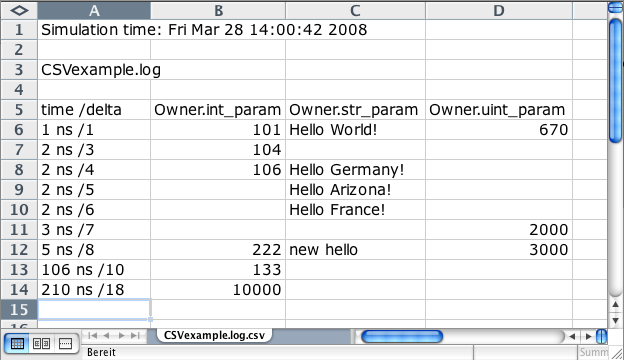
\includegraphics[width=15cm]{./images/csvExcelExample}}
	\caption{CSV ouput plugin Excel example}
	\label{fig:GAVcsvExcelExample}
\end{figure}


%%%%
\subsection{SCV-stream Output Plugin}
\label{GAVOPscv}

\begin{itemize}
  \item Include \Datei{greencontrol/analysis\_scv\_outputplugin.h}
  \item Implementation see file \Datei{SCV\_OutputPlugin}
  \item Identify this output plugin with {\sffamily gs::av::SCV\_STREAM\_OUT}, \newline
           id ({\sffamily OutputPluginType}) = 5.
\end{itemize}

The SCV output plugin (\lstinline|SCV_OutputPlugin|) outputs parameter changes to a stream of the SystemC Verification Standard (SCV). This standard stream can be used as an input to several vendor tools (such as CoWare and Mentor).

 This output plugin exports the registered
 parameter changes to an {\em SCV stream} named \mbox{\sffamily GreenAVstream\_$<$OutputPluginName$>$}. The constructor string parameter is the {\sffamily OutputPluginName}. Each
 parameter gets its own transaction generator. When a parameter changes, the previous
 transaction is ended and a new one with the new value is started. Accordingly a 
 transaction represents the time where the value of a parameter remains unchanged.

 The database that should be written to can be chosen in the static function 
 \lstinline|init_scv_recording()| (see file \Datei{SCV\_OutputPlugin.h}).

The output plugin's {\em default database} is a text file which is the default database in the SCV framework. The SCV stream output is written to the file \Datei{transaction\_text\_db}.  Add \#define areas to use other databases (like ModelSim).

There are some options to change the output plugin's behavior to be able to support a wide range of external tools reading the SCV stream. These options can be changed in the define area at the top of the file \Datei{SCV\_OutputPlugin.h}.

\begin{itemize}

  \item  The default is to use only one globals database for all SCV output plugin instances. If there is a database type that is able to handle more than one database, undefine the \newline
  \lstinline[language=TeX]|#define ONLY_ONE_GLOBAL_DATABASE|.

  \item  If a tool or database is only able to handle one stream, use the \lstinline[language=TeX]|#define ONLY_ONE_GLOBAL_STREAM| (defined by default). \newline
 Then all \lstinline|SCV_OutputPlugin| instances write to the same stream.

  \item  The OutputPlugin is able to create transactions with values of the type {\sffamily string} (default)
 The user may set \lstinline[language=TeX]|#define USE_CORRECT_TYPE_TRANSACTIONS true|
 to enable transactions containing values of the correct type (as long as the type is listed in the enum
 {\sffamily gs::cnf::Param\_type} and is implemented here). This is slower because of 
 some additional switch statements and casts.

\end{itemize}

The files \Datei{AVscvAnalyserTool.*} in the example \Verzeichnis{greencontrol/examples/gav\_simple} create SCV output streams.


\ZwischenUberschrift{Experience with Mentor Graphics ModelSim}
{\sffamily ModelSim} (Mentor Graphics) has the ability to run SystemC simulations and to show the results graphically. GreenBus and \GreenControl (including \GreenConfig and \GreenAV) can be compiled with Mentor's {\sffamily sccom} compiler and can be run with the {\sffamily vsim} simulator.

Mentor's SCV implementation does not support string data types in transactions being recorded in an SCV stream. Accordingly the SCV output plugin has to use the {\sffamily \small USE\_CORRECT\_TYPE\_TRANSACTIONS} define and cannot show string parameters. So the visualization is restricted to the data types listed in the enumeration {\sffamily gs::cnf::Param\_type} and implemented in the plugin.

The SCV output plugin has an \lstinline|init_recording| function which automatically uses ModelSim special code when compiled with the ModelSim sccom compiler. In the define section there is an \lstinline|ifdef| for ModelSim which automatically sets the correct behavior.
  
These steps have to be performed when simulating with ModelSim:
\begin{itemize}
  \item Start the simulation ({\em Important!} The transaction stream does not occur before simulation is running and has created the stream!)
  \item View the recorded SCV transactions by right clicking on the module which contains the stream and selecting {\sffamily Add $\rightarrow$ Add All Signals to Wave}. %(TODO: This should be the GAV plugin named 'AnalysisPlugin' but is is the module which initiated the first observation of this output plugin.) 
\end{itemize}


\ZwischenUberschrift{Experience with CoWare}
Experiments with the {\sffamily CoWare Platform Architect}:

To use the CoWare settings, \#define \lstinline|CoWare|. The SCV output plugin has a special define area in its \lstinline|init_recording| function for the CoWare tool. In the define section there is an \lstinline|ifdef| for CoWare which automatically sets the correct behavior.


%%%%
\subsection{How to implement an Output Plugin}
\label{GAVimplementOP}

This is a short introduction how to implement a new output plugin. For a simple example see the STDOUT output plugin in file \Datei{Stdout\_OutputPlugin.h} (see section \ref{GAVOPstdout}).

\begin{itemize}
  \item Outside the class (but in same namespace) specify the project-wide unique id and convenience name with the macro {\sffamily GAV\_REGISTER\_PLUGIN(unique\_id, convenience\_variable, class\_name)}. \newline
     Example:
    \begin{lstlisting}
GAV_REGISTER_PLUGIN(10, MY_NEW_OUT, MyNew_OutputPlugin);
    \end{lstlisting}
  \item Inherit \lstinline|OuputPlugin_base| which provides most functionality expect the output itself.
  \item Do not implement the empty constructor.
  \item Implement the constructor taking a name and an event listener and forward the event listener to the base class:
    \begin{lstlisting}
MyNew_OutputPlugin ( const char* unused, 
                      event_listener<OutputPlugin_base> *ev_listn)
 : OutputPlugin_base(ev_listn)
    \end{lstlisting}
  \item Implement the callback function and make sure to remove a parameter being observed by the output plugin when is is being destroyed. Guard the output by checking \lstinline|is_running|.
    \begin{lstlisting}
void config_callback(gs_param_base &par) {
  if (par.is_destructing()) {
    remove(par);
  }  else if (is_running) {
    // Do the output
  }
}
    \end{lstlisting}
  \item Implement the output within the callback function (previous bullet point). Use the functions the \lstinline|gs_param_base| provides or cast to the actual \lstinline|gs_param<type>| type (see \GreenConfig User's Guide\footnote{\hypertarget{GCnfUsersGuide08target}{\GreenConfig User's Guide}: \url{http://www.greensocs.com/projects/GreenControl/GreenConfig}}).
    \begin{lstlisting}
par.getName();
par.getString(); 
    \end{lstlisting}
  \item Create a member representing the new output plugin in the enum {\sffamily OutputPluginType} in file \Datei{gav\_datatypes.h}.
    \begin{lstlisting}
enum OutputPluginType {
  [... other members ...],
  // Short explanation of my outp.pl.
  MYNEW_OUTPUT_PLUGIN
}
    \end{lstlisting}
  \item Add the new output plugin to the GAV plugin's \lstinline|outputPluginFabricCreator| function (file \Datei{gav\_plugin.h}) by adding a switch case. The case is the enum member being created at the preceding bullet point.
    \begin{lstlisting}
case MYNEW_OUTPUT_PLUGIN:
{
  // create MyNew output plugin
  op = new MyNew_OutputPlugin(constructParam, &m_OutpPl_event_listener);
  break;
}
    \end{lstlisting}


\end{itemize}

\Note{Advanced Note}{Write an Output Plugin from scratch}{
  When writing a completely new output plugin at least the interface {\sffamily OuputPlugin\_if} has to be implemented. The constructor should get (but needs not) the string given by the user, transmitted over the transaction.
}